\chapter{Les réactions chimiques~: réactifs et produits}\label{ch:g7:chemical-reactions}

Du charbon de bois rougeoie dans un barbecue. Une heure plus tard, il ne
reste presque rien des morceaux noirs --- un peu de cendre grise, et la
chaleur qui a cuit le repas. Où le carbone noir est-il passé~? Il n'a
pas disparu~: il a rencontré le dioxygène de l'\omterm{def:g4:air-a-mixture-of-gases:air}{air} et il est devenu un
nouveau gaz, invisible. Avec les \omterm{def:g7:atoms-and-molecules:atom}{atomes} et les \omterm{def:g7:atoms-and-molecules:molecule}{molécules} en main, on
peut maintenant dire exactement ce qui se passe lors d'une telle
transformation.

\begin{recall}
Au cours d'une \omterm{def:g5:irreversible-changes:chemical-change}{transformation chimique}, de nouvelles substances
apparaissent et il n'y a pas de chemin de retour simple
(\cref{ch:g5:irreversible-changes}). L'eau de chaux se trouble avec le
dioxyde de carbone, le sulfate de cuivre anhydre bleuit avec l'eau
(\cref{ch:g7:identifying-substances}). Toute la matière est faite
d'\omterm{def:g7:atoms-and-molecules:atom}{atomes}, qui se regroupent en \omterm{def:g7:atoms-and-molecules:molecule}{molécules}~; une formule comme \ce{CO2}
énumère les \omterm{def:g7:atoms-and-molecules:atom}{atomes} d'une \omterm{def:g7:atoms-and-molecules:molecule}{molécule} (\cref{ch:g7:atoms-and-molecules}).
\end{recall}

\begin{omfigure}
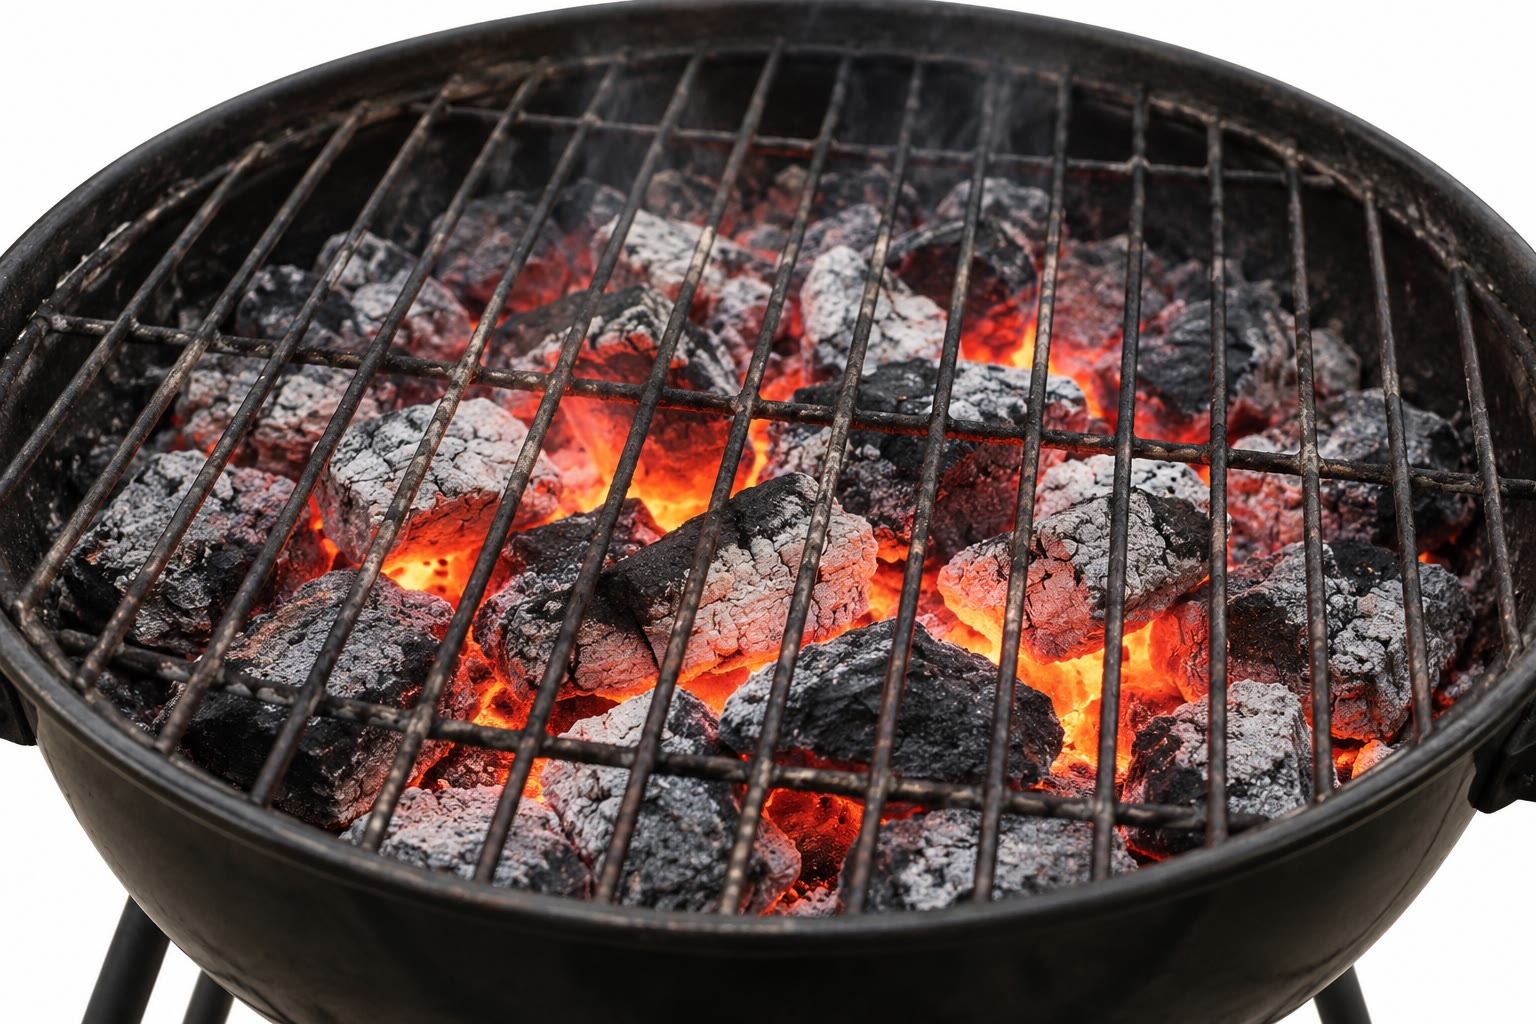
\includegraphics[width=0.55\linewidth]{images/book1/ai/g7-charcoal-bbq.jpg}

{\small Du charbon de bois rougeoyant~: le carbone réagit avec le
dioxygène de l'\omterm{def:g4:air-a-mixture-of-gases:air}{air}.}
\end{omfigure}

\section{Transformations physiques et chimiques}

\begin{definition}[Transformation physique]\label{def:g7:chemical-reactions:physical-transformation}
Une \emph{transformation physique}\index{transformation physique}
change l'état ou l'arrangement de la matière sans changer les \omterm{def:g6:pure-substances-and-mixtures:species}{espèces
chimiques}~: la fusion, la solidification, l'ébullition, la dissolution,
le \omterm{def:g6:pure-substances-and-mixtures:mixture}{mélange}. Les mêmes espèces sont présentes avant et après~; seuls leur
forme ou leur arrangement ont changé.
\end{definition}

\begin{example}[L'eau, de trois façons]\label{ex:g7:chemical-reactions:water}
La glace qui fond en eau, l'eau qui bout en vapeur d'eau et le sel qui
\omterm{def:g2:mixing-and-dissolving:dissolve}{se dissout} dans l'eau sont des \omterm{def:g7:chemical-reactions:physical-transformation}{transformations physiques}~: avant comme
après, il y a des \omterm{def:g7:atoms-and-molecules:molecule}{molécules} d'eau (et du sel). En zoomant, on voit les
mêmes \omterm{def:g7:atoms-and-molecules:molecule}{molécules}~; seules leur disposition et la façon dont elles
bougent ont changé.
\end{example}

\begin{proposition}[Transformation chimique]\label{prop:g7:chemical-reactions:chemical}
Au cours d'une \omterm{def:g5:irreversible-changes:chemical-change}{transformation chimique}, certaines \omterm{def:g6:pure-substances-and-mixtures:species}{espèces chimiques}
disparaissent et de nouvelles apparaissent. On la distingue d'une
\omterm{def:g7:chemical-reactions:physical-transformation}{transformation physique} par ses \omterm{def:g7:chemical-reactions:reactant}{produits}~: des espèces nouvelles, que
l'on peut mettre en évidence par des \omterm{def:g7:identifying-substances:characteristic-test}{tests caractéristiques}.
\end{proposition}

\begin{omfigure}
\begin{tikzpicture}[font=\small, level distance=1.5cm,
    box/.style={draw=omDef, fill=omDef!6, rounded corners=2pt, align=center,
      inner sep=4pt},
    level 1/.style={sibling distance=6.6cm},
    edge from parent/.style={draw, thick, omDef, ->}]
  \node[box] {une transformation de la matière}
    child {node[box, text width=5.2cm] {\textbf{physique}~: les mêmes espèces\\
      avant et après\\ \footnotesize fusion, ébullition, dissolution, mélange}}
    child {node[box, draw=omProp, fill=omProp!6, text width=5.2cm]
      {\textbf{chimique}~: des espèces disparaissent,\\ de nouvelles espèces apparaissent\\
      \footnotesize combustion, rouille, cuisson}};
\end{tikzpicture}

{\small Deux sortes de transformations.}
\end{omfigure}

\section{Réactifs et produits}

\begin{definition}[Réaction chimique]\label{def:g7:chemical-reactions:reaction}
Une \emph{réaction chimique}\index{reaction chimique@réaction chimique} est le modèle
qu'utilisent les chimistes pour décrire une \omterm{def:g5:irreversible-changes:chemical-change}{transformation chimique}~:
elle énumère les espèces consommées et les espèces formées.
\end{definition}

\begin{definition}[Réactifs et produits]\label{def:g7:chemical-reactions:reactant}
Les espèces consommées au cours d'une \omterm{def:g7:chemical-reactions:reaction}{réaction chimique} sont les
\emph{réactifs}\index{reactif@réactif}~; les espèces formées sont les
\emph{produits}\index{produit}.
\end{definition}

\begin{example}[Le carbone qui brûle dans le dioxygène]\label{ex:g7:chemical-reactions:carbon}
Quand le charbon de bois \omterm{def:g4:what-a-fire-needs:burning}{brûle}, les \omterm{def:g7:chemical-reactions:reactant}{réactifs} sont le carbone (le
charbon) et le dioxygène (de l'\omterm{def:g4:air-a-mixture-of-gases:air}{air}). Le \omterm{def:g7:chemical-reactions:reactant}{produit} est le dioxyde de
carbone~: agité avec de l'eau de chaux, le gaz resté dans le flacon la
trouble.
\end{example}

\begin{inthelab}[Du charbon de bois dans un flacon de dioxygène]
L'enseignant chauffe un petit morceau de charbon de bois jusqu'à ce
qu'il rougeoie, sur un têt à \omterm{def:g4:what-a-fire-needs:burning}{combustion}, puis le descend dans un flacon
de dioxygène. Le charbon brille beaucoup plus fort que dans l'\omterm{def:g4:air-a-mixture-of-gases:air}{air} et
rapetisse jusqu'à disparaître. On couvre le flacon, on y verse un peu
d'eau de chaux et on agite~: elle se trouble. Le carbone et le dioxygène
ont été consommés~; du dioxyde de carbone s'est formé.
\end{inthelab}

\begin{omfigure}
\begin{tikzpicture}[font=\small, scale=1.3]
  \pic[transform shape] at (0,0) {gasjaropen={0}{white}};
  \fill[omWater!60] (-0.68,2.62) rectangle (0.68,2.7);
  \draw[omGlass, line width=0.4pt] (-0.68,2.62) rectangle (0.68,2.7);
  \draw[black!60, line width=1.2pt] (0.15,2.7) -- (0.15,3.6) -- (1.2,3.6);
  \draw[black!60, line width=1.2pt] (0.15,2.7) -- (0.15,1.2);
  \fill[black!60] (-0.12,1.12) rectangle (0.32,1.2);
  \fill[red!70!black] (0.0,1.32) circle (0.13);
  \fill[orange!90!yellow] (0.0,1.32) circle (0.08);
  \draw[<-, omProp, thick] (0.15,1.35) -- (1.5,1.6) node[right, text=black]
    {charbon rougeoyant (carbone)};
  \draw[<-, omProp, thick] (-0.35,2.1) -- (1.5,2.3) node[right, text=black]
    {dioxygène};
  \draw[<-, omProp, thick] (0.6,2.66) -- (1.5,2.95) node[right, text=black]
    {couvercle};
  \draw[<-, omProp, thick] (0.15,3.1) -- (1.5,3.6) node[right, text=black]
    {têt à combustion};
\end{tikzpicture}

{\small Du charbon rougeoyant descendu sur un têt dans un flacon de
dioxygène \omterm{def:g4:what-a-fire-needs:burning}{brûle} vivement~: le carbone et le dioxygène réagissent pour
former du dioxyde de carbone.}
\end{omfigure}

\begin{example}[La laine d'acier]\label{ex:g7:chemical-reactions:steel-wool}
Un tampon de laine d'acier fine, faite surtout de fer, peut \omterm{def:g4:what-a-fire-needs:burning}{brûler} dans
l'\omterm{def:g4:air-a-mixture-of-gases:air}{air} en lançant des gerbes d'étincelles. Les \omterm{def:g7:chemical-reactions:reactant}{réactifs} sont le fer et le
dioxygène~; le \omterm{def:g7:chemical-reactions:reactant}{produit} est un solide sombre et friable, un oxyde de fer.
\end{example}

\begin{omfigure}
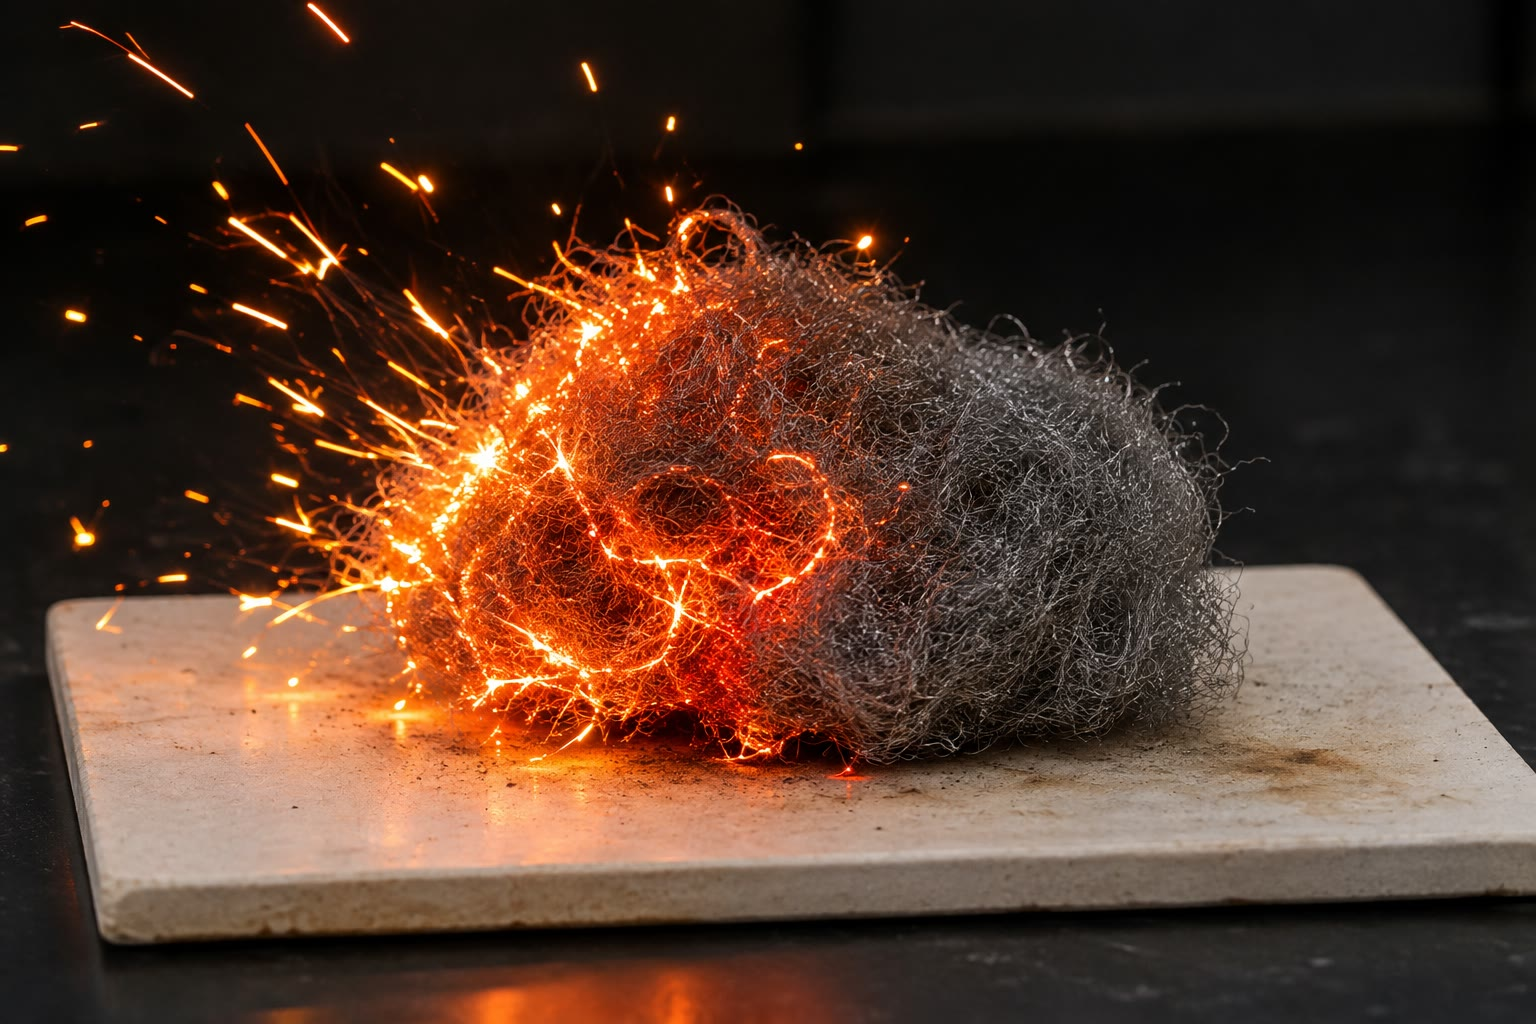
\includegraphics[width=0.5\linewidth]{images/book1/ai/g7-steel-wool-burning.jpg}

{\small De la laine d'acier qui \omterm{def:g4:what-a-fire-needs:burning}{brûle} au laboratoire~: le fer et le
dioxygène réagissent.}
\end{omfigure}

\section{L'équation en mots}

\begin{definition}[Équation en mots]\label{def:g7:chemical-reactions:word-equation}
Une \emph{équation en mots}\index{equation en mots@équation en mots} écrit une \omterm{def:g7:chemical-reactions:reaction}{réaction
chimique} avec des mots~: les noms des \omterm{def:g7:chemical-reactions:reactant}{réactifs} à gauche, reliés par $+$,
une flèche, et les noms des \omterm{def:g7:chemical-reactions:reactant}{produits} à droite. La flèche se lit
«~réagissent pour donner~».
\end{definition}

\begin{example}[Trois équations en mots]\label{ex:g7:chemical-reactions:three}
\begin{center}
\begin{tabular}{l}
carbone $+$ dioxygène $\longrightarrow$ dioxyde de carbone\\[2pt]
méthane $+$ dioxygène $\longrightarrow$ dioxyde de carbone $+$ eau\\[2pt]
fer $+$ dioxygène $\longrightarrow$ oxyde de fer
\end{tabular}
\end{center}
\end{example}

\begin{method}[Écrire une équation en mots]\label{met:g7:chemical-reactions:write}
\begin{enumerate}
  \item Trouver les \omterm{def:g7:chemical-reactions:reactant}{réactifs}~: les espèces qui disparaissent.
  \item Trouver les \omterm{def:g7:chemical-reactions:reactant}{produits}~: les espèces nouvelles, identifiées par des
        tests.
  \item Écrire les \omterm{def:g7:chemical-reactions:reactant}{réactifs} à gauche, les \omterm{def:g7:chemical-reactions:reactant}{produits} à droite, avec une
        flèche entre eux~; jamais un signe égal.
\end{enumerate}
Une espèce présente qui ne participe pas à la réaction --- le diazote de
l'\omterm{def:g4:air-a-mixture-of-gases:air}{air} qui entoure une flamme --- ne s'écrit pas.
\end{method}

\section{Une réaction réarrange les atomes}

\begin{proposition}[Les atomes sont réarrangés]\label{prop:g7:chemical-reactions:rearranged}
Au cours d'une \omterm{def:g7:chemical-reactions:reaction}{réaction chimique}, les \omterm{def:g7:atoms-and-molecules:molecule}{molécules} des \omterm{def:g7:chemical-reactions:reactant}{réactifs} sont
brisées et leurs \omterm{def:g7:atoms-and-molecules:atom}{atomes} s'assemblent autrement pour construire les
\omterm{def:g7:atoms-and-molecules:molecule}{molécules} des \omterm{def:g7:chemical-reactions:reactant}{produits}. Les \omterm{def:g7:atoms-and-molecules:atom}{atomes} eux-mêmes ne sont ni créés ni
détruits~: les mêmes \omterm{def:g7:atoms-and-molecules:atom}{atomes}, en mêmes nombres, sont présents avant et
après.
\end{proposition}

\begin{example}[La combustion du méthane, molécule par molécule]\label{ex:g7:chemical-reactions:methane}
Quand le méthane d'une cuisinière \omterm{def:g4:what-a-fire-needs:burning}{brûle}, une \omterm{def:g7:atoms-and-molecules:molecule}{molécule} de méthane
\ce{CH4} rencontre deux \omterm{def:g7:atoms-and-molecules:molecule}{molécules} de dioxygène \ce{O2}. Leurs \omterm{def:g7:atoms-and-molecules:atom}{atomes} se
réarrangent en une \omterm{def:g7:atoms-and-molecules:molecule}{molécule} de dioxyde de carbone \ce{CO2} et deux
\omterm{def:g7:atoms-and-molecules:molecule}{molécules} d'eau \ce{H2O}. Avant~: 1 \omterm{def:g7:atoms-and-molecules:atom}{atome} de carbone, 4 d'hydrogène et 4
d'oxygène. Après~: 1 de carbone, 4 d'hydrogène, et $2 + 2 = 4$
d'oxygène. Rien ne se perd, rien n'apparaît de nulle part.
\end{example}

\begin{omfigure}
\begin{tikzpicture}[font=\small]
  % methane
  \begin{scope}[xshift=0cm]
    \node[aC] (c) at (0,0) {};
    \node[aH] (h1) at (0,0.78) {}; \node[aH] (h2) at (-0.74,-0.3) {};
    \node[aH] (h3) at (0.74,-0.3) {}; \node[aH] (h4) at (0.2,-0.68) {};
    \begin{scope}[on background layer]
      \foreach \h in {h1,h2,h3,h4} \draw[bond] (c.center) -- (\h.center);
    \end{scope}
    \node at (0,-1.2) {1 méthane};
  \end{scope}
  \node at (1.45,0) {$+$};
  % two oxygen molecules
  \foreach \y in {0.45,-0.45} {
    \node[aO] (a) at (2.4,\y) {}; \node[aO] (b) at (3.05,\y) {};
    \begin{scope}[on background layer]
      \draw[bond, line width=1.1pt] ([yshift=1.6pt]a.center) -- ([yshift=1.6pt]b.center);
      \draw[bond, line width=1.1pt] ([yshift=-1.6pt]a.center) -- ([yshift=-1.6pt]b.center);
    \end{scope}
  }
  \node at (2.72,-1.2) {2 dioxygène};
  \draw[->, thick, omProp] (3.8,0) -- (5.0,0);
  % carbon dioxide
  \begin{scope}[xshift=6.3cm]
    \node[aO] (a) at (-0.8,0) {}; \node[aC] (c) at (0,0) {}; \node[aO] (b) at (0.8,0) {};
    \begin{scope}[on background layer]
      \foreach \d in {-1.6,1.6} {
        \draw[bond, line width=1.1pt] ([yshift=\d pt]a.center) -- ([yshift=\d pt]c.center);
        \draw[bond, line width=1.1pt] ([yshift=\d pt]c.center) -- ([yshift=\d pt]b.center);}
    \end{scope}
    \node at (0,-1.2) {1 dioxyde de carbone};
  \end{scope}
  \node at (7.8,0) {$+$};
  % two water molecules
  \foreach \x in {8.9,10.6} {
    \node[aO] (o) at (\x,0.2) {};
    \node[aH] (p) at (\x-0.58,-0.25) {}; \node[aH] (q) at (\x+0.58,-0.25) {};
    \begin{scope}[on background layer]
      \draw[bond] (o.center) -- (p.center); \draw[bond] (o.center) -- (q.center);
    \end{scope}
  }
  \node at (9.75,-1.2) {2 eau};
  % atom counts
  \node[align=center, font=\footnotesize] at (1.5,-2.0) {avant~: 1 C, 4 H, 4 O};
  \node[align=center, font=\footnotesize] at (8.5,-2.0) {après~: 1 C, 4 H, 4 O};
\end{tikzpicture}

{\small La \omterm{def:g4:what-a-fire-needs:burning}{combustion} du méthane, dessinée avec des modèles
moléculaires~: les \omterm{def:g7:atoms-and-molecules:atom}{atomes} des \omterm{def:g7:chemical-reactions:reactant}{réactifs} se réarrangent pour former les
\omterm{def:g7:chemical-reactions:reactant}{produits}. On compte les mêmes \omterm{def:g7:atoms-and-molecules:atom}{atomes} avant et après.}
\end{omfigure}

\begin{remark}[Compter les molécules]\label{rem:g7:chemical-reactions:counting}
L'\omterm{def:g7:chemical-reactions:word-equation}{équation en mots} ne dit pas combien de \omterm{def:g7:atoms-and-molecules:molecule}{molécules} réagissent~: pour
cela, on écrit l'équation avec des formules précédées de nombres. Écrire
de telles équations, et trouver les bons nombres, est l'objet d'un
chapitre suivant.
\end{remark}

\section{Exercices}

\begin{exercise}[$\star$]\label{exo:g7:chemical-reactions:1}
\omterm{def:g7:chemical-reactions:physical-transformation}{Transformation physique} ou chimique~? La glace qui fond, une allumette
qui \omterm{def:g4:what-a-fire-needs:burning}{brûle}, le sucre qui \omterm{def:g2:mixing-and-dissolving:dissolve}{se dissout}, le pain qui grille, un clou qui
rouille.
\end{exercise}

\begin{exercise}[$\star$]\label{exo:g7:chemical-reactions:2}
Que sont les \omterm{def:g7:chemical-reactions:reactant}{réactifs} et les \omterm{def:g7:chemical-reactions:reactant}{produits} d'une \omterm{def:g7:chemical-reactions:reaction}{réaction chimique}~?
\end{exercise}

\begin{exercise}[$\star$]\label{exo:g7:chemical-reactions:3}
Écris l'\omterm{def:g7:chemical-reactions:word-equation}{équation en mots} de la \omterm{def:g4:what-a-fire-needs:burning}{combustion} du carbone dans le dioxygène.
\end{exercise}

\begin{exercise}[$\star$]\label{exo:g7:chemical-reactions:4}
Dans l'\omterm{def:g7:chemical-reactions:word-equation}{équation en mots} «~fer $+$ dioxygène $\longrightarrow$ oxyde de
fer~», nomme les \omterm{def:g7:chemical-reactions:reactant}{réactifs} et le \omterm{def:g7:chemical-reactions:reactant}{produit}.
\end{exercise}

\begin{exercise}[$\star\star$]\label{exo:g7:chemical-reactions:5}
Quand le méthane \omterm{def:g4:what-a-fire-needs:burning}{brûle}, un verre froid tenu au-dessus de la flamme se
couvre de buée, et le gaz recueilli trouble l'eau de chaux. Quels
\omterm{def:g7:chemical-reactions:reactant}{produits} ces deux tests mettent-ils en évidence~?
\end{exercise}

\begin{exercise}[$\star\star$]\label{exo:g7:chemical-reactions:6}
Le zinc réagit avec l'acide chlorhydrique~: le zinc disparaît, des
bulles de dihydrogène se dégagent, et du chlorure de zinc reste dans la
solution. Écris l'\omterm{def:g7:chemical-reactions:word-equation}{équation en mots}.
\end{exercise}

\begin{exercise}[$\star\star$]\label{exo:g7:chemical-reactions:7}
Regarde la figure des modèles de la \omterm{def:g4:what-a-fire-needs:burning}{combustion} du méthane. Compte les
\omterm{def:g7:atoms-and-molecules:atom}{atomes} d'hydrogène avant et après la réaction.
\end{exercise}

\begin{exercise}[$\star\star$]\label{exo:g7:chemical-reactions:8}
Pourquoi la dissolution du sel dans l'eau n'est-elle pas une \omterm{def:g7:chemical-reactions:reaction}{réaction
chimique}, bien que le sel disparaisse à la vue~?
\end{exercise}

\begin{exercise}[$\star\star$]\label{exo:g7:chemical-reactions:9}
Une bûche se réduit en brûlant à un petit tas de cendre. Explique, en
employant le mot «~\omterm{def:g7:chemical-reactions:reactant}{produits}~», pourquoi la cendre est tellement plus
légère que la bûche.
\end{exercise}

\begin{exercise}[$\star\star$]\label{exo:g7:chemical-reactions:10}
Le dihydrogène \omterm{def:g4:what-a-fire-needs:burning}{brûle} dans le dioxygène en donnant uniquement de l'eau.
Écris l'\omterm{def:g7:chemical-reactions:word-equation}{équation en mots}, et dis quel test permettrait d'identifier le
\omterm{def:g7:chemical-reactions:reactant}{produit}.
\end{exercise}

\begin{exercise}[$\star\star\star$]\label{exo:g7:chemical-reactions:11}
Deux \omterm{def:g7:atoms-and-molecules:molecule}{molécules} de dihydrogène \ce{H2} réagissent avec une \omterm{def:g7:atoms-and-molecules:molecule}{molécule} de
dioxygène \ce{O2} pour donner deux \omterm{def:g7:atoms-and-molecules:molecule}{molécules} d'eau \ce{H2O}. Compte les
\omterm{def:g7:atoms-and-molecules:atom}{atomes} de chaque sorte avant et après, et montre qu'aucun n'a été créé
ni détruit.
\end{exercise}

\begin{exercise}[$\star\star\star$]\label{exo:g7:chemical-reactions:12}
Un élève représente la \omterm{def:g4:what-a-fire-needs:burning}{combustion} du carbone ainsi~: un \omterm{def:g7:atoms-and-molecules:atom}{atome} de carbone
$+$ une \omterm{def:g7:atoms-and-molecules:molecule}{molécule} de dioxygène $\longrightarrow$ une \omterm{def:g7:atoms-and-molecules:molecule}{molécule} de dioxyde
de carbone et un \omterm{def:g7:atoms-and-molecules:atom}{atome} d'oxygène en trop. Qu'est-ce qui ne va pas dans
ce dessin~? Décris en mots le dessin correct.
\end{exercise}

\section{Problème~: au cœur d'une flamme de gazinière}

\begin{problem}[{Problème du week-end --- ce qui brûle dans la flamme d'une
gazinière, ce que cela produit, et combien de molécules y prennent part}]
\label{pb:g7:chemical-reactions:1}
Le gaz d'une cuisinière est surtout du méthane, \ce{CH4}. Dans sa flamme
bleue, le méthane réagit avec le dioxygène de l'\omterm{def:g4:air-a-mixture-of-gases:air}{air}. Au laboratoire,
l'enseignant tient quelques secondes un bécher froid et sec, retourné,
au-dessus d'une telle flamme, puis le remet à l'endroit, y verse un peu
d'eau de chaux et agite.

\medskip
\noindent\textbf{Partie I --- \omterm{def:g7:chemical-reactions:reactant}{Réactifs} et \omterm{def:g7:chemical-reactions:reactant}{produits}.}
\begin{enumerate}
  \item Nomme les deux \omterm{def:g7:chemical-reactions:reactant}{réactifs} de cette réaction.
  \item Des gouttelettes apparaissent à l'intérieur du bécher froid~; une
        goutte bleuit le sulfate de cuivre anhydre. Quel \omterm{def:g7:chemical-reactions:reactant}{produit} cela
        met-il en évidence~?
  \item L'eau de chaux se trouble. Quel autre \omterm{def:g7:chemical-reactions:reactant}{produit} cela met-il en
        évidence~?
  \item L'\omterm{def:g4:air-a-mixture-of-gases:air}{air} contient aussi du diazote, qui traverse la flamme sans
        changer. Le diazote est-il un \omterm{def:g7:chemical-reactions:reactant}{réactif}~? Doit-il figurer dans
        l'\omterm{def:g7:chemical-reactions:word-equation}{équation en mots}~?
\end{enumerate}

\medskip
\noindent\textbf{Partie II --- L'\omterm{def:g7:chemical-reactions:word-equation}{équation en mots}.}
\begin{enumerate}[resume]
  \item Écris l'\omterm{def:g7:chemical-reactions:word-equation}{équation en mots} de la réaction.
  \item La \omterm{def:g4:what-a-fire-needs:burning}{combustion} du méthane est-elle une \omterm{def:g7:chemical-reactions:physical-transformation}{transformation physique} ou
        chimique~? Donne deux raisons.
  \item Écris les formules des quatre espèces de la réaction.
\end{enumerate}

\medskip
\noindent\textbf{Partie III --- Compter les \omterm{def:g7:atoms-and-molecules:molecule}{molécules}.}
Chaque \omterm{def:g7:atoms-and-molecules:molecule}{molécule} de méthane qui \omterm{def:g4:what-a-fire-needs:burning}{brûle} réagit avec deux \omterm{def:g7:atoms-and-molecules:molecule}{molécules} de
dioxygène, et donne une \omterm{def:g7:atoms-and-molecules:molecule}{molécule} de dioxyde de carbone et deux \omterm{def:g7:atoms-and-molecules:molecule}{molécules}
d'eau.
\begin{enumerate}[resume]
  \item Compte les \omterm{def:g7:atoms-and-molecules:atom}{atomes} de carbone, d'hydrogène et d'oxygène dans une
        \omterm{def:g7:atoms-and-molecules:molecule}{molécule} de méthane et deux \omterm{def:g7:atoms-and-molecules:molecule}{molécules} de dioxygène, ensemble.
  \item Compte-les dans une \omterm{def:g7:atoms-and-molecules:molecule}{molécule} de dioxyde de carbone et deux
        \omterm{def:g7:atoms-and-molecules:molecule}{molécules} d'eau, ensemble. Que remarques-tu~?
  \item La flamme \omterm{def:g4:what-a-fire-needs:burning}{brûle} 10 \omterm{def:g7:atoms-and-molecules:molecule}{molécules} de méthane. Combien de \omterm{def:g7:atoms-and-molecules:molecule}{molécules} de
        dioxygène consomme-t-elle~?
  \item Combien de \omterm{def:g7:atoms-and-molecules:molecule}{molécules} de dioxyde de carbone produit-elle~?
  \item Combien de \omterm{def:g7:atoms-and-molecules:molecule}{molécules} d'eau produit-elle~?
\end{enumerate}
\end{problem}
